\logg{Onsdag 18. September}{10:00 til 14:00 (4 timer)}{
Møtte opp klokken 10:00 for å fortsette forbredelser til fremtidig arbeid. Her begynte studenten å bygge en postgres database på laptopen som ble utdelt. Der fikk studenten en \textit{dump} fil, hvor det ligger mye data som skal bli brukt i prosjektet. Studenten forsøkte å bygge databasen med hjelp fra DBeaver programmet som ble lastet ned forrige uke, men dette viste seg å være en utfordring. Det endte med at studenten skapte en database ved hjelp av kommandolinjen. Når studenten skulle \textit{restore} dataen fra dump filen, oppstod det noen problemer. Studenten valgte da å gjøre litt research på hva man kan gjøre for å gjenopprette dataen. \\

Etter flere forsøk uten noen framgang, valgte studenten å se mer på \textit{trace-insight} applikasjonen. Her var det den \textit{README.md} fil hvor det var instrukser på hva man må gjøre for å få applikasjonen til å kjøre. Applikasjonen bruker bruker fire teknologier. \textit{Gardle}, \textit{Node}, \textit{Docker}, og \textit{Postgres}. Det var skrevet i dokumentasjonen at man måtte starte starte backend og fortsend for å bruke applikasjonen i localhost. Npr studenten skulle starte backend feilet systemet å bygge den. Studenten prøvde da å starte froentend for å se om den måtte kjøre først. Frontend fungerte, men applikasjonen var helt hvit. Dette var grunnet at hvis backend ikke kjører, skal ingenting vises. Studenten forsøkte da å installere Gradle og forstatte å lese dokumentasjon på denne teknologien for å prøve å finne feilen. \\

Med lite progresjon, bestemte eleven seg for å lese seg opp på \textit{abc-analyse} og dokumentasjon på en annen applikasjon (som fungerte).

\begin{figure}[H]
\centering
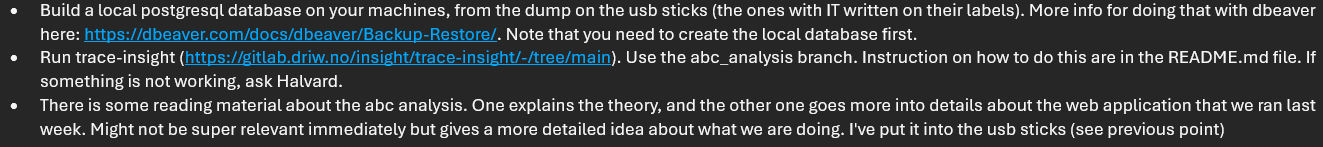
\includegraphics[width=1\linewidth]{ukentlige logger/images/uke 2/email_instructions_week_2.png}
\caption{\label{fig:downloads}E-post med oppgaver som må gjøres.}
\end{figure}

Dette forstatte ut dagen til klokken ble 14:00 da studenten måtte dra for å rekke en forelesing.
}\\\\\\